\subsection{Regression}
\label{sec:results-regression}
The objective of the regression task is to perform localization with performance comparable to GPS system. The parameters of the training had to be tuned for the network to perform at its best for the regression task.

The layers of the network are initialized using normal distributions. The initialization variances had to be changed from 0.01 to 0.1 for Conv1 and to 0.05 for Conv2, Conv3, Conv4 and Conv5, so that the weights are big enough to propagate information through the network while still ensuring convergence.
The initial learning rate and its evolution policy heavily depends on the loss which is used. For the regression task, very high values and a diverging behaviour were observed with the Euclidean loss at the beginning of the training. The initial learning rate had to be decreased to avoid these effects. The learning rate policy was set to the "step" policy from Caffe and it was chosen to decrease the learning rate by half every 25 000 iterations. In our case this corresponds to the number of iterations required to observe the stabilization of the loss after each exponential decrease.

In this context, we tested three different approaches.  The first one consists in training every layer with the same learning rate. The second one consists in fine-tuning the learning rate of each layer differently based on the results given by the first approach. The third one consists in loading the weights of the convolution layers from the classification training. In order to compare our results with those three approaches, we refer to the following loss function :

\begin{equation} 
Loss = \frac{0.5}{scale^{2}}*\sum_{i=1,\ 4}(label_{i}-prediction_{i})^{2}
\end{equation}

The first approach allowed to achieve an average error of 19.3 meters per label as it is shown in fig.~\ref{1apploss}.a. The loss computed on the test dataset is plotted in green and the loss computed on the train dataset is plotted in blue. However after the training, the convolution layers filters did not exhibit any specific features (fig.~\ref{1appfilter}.a). Thus, it appears that the regression was only supported by the fully connected layers. In our case where the goal is to build a seasonal invariant representation of natural scenes this approach did not reach our expectations. 

The second approach led us to consider the difference of behavior of the fully-connected layers regarding the sensitivity to learning rate. By decreasing the learning rate of those layers, we forced the convolution layers to take part in the regression. This method resulted in being more successful than the previous one. The best average error we achieved was 18.3 meters (fig.~\ref{2apploss}.b). Some natural environment features can be identified in the convolution filters (fig.~\ref{2appfilter}.b).

The last approach was used the same learning rate settings as the first approach. It was observed that the convolution weights decreased during the training and ended with a distribution similar to the second approach. The best average error achieved was 20.9 (fig.~\ref{3apploss}.c). However the convolution filters retrieved exhibited different structures than the second approach (fig.~\ref{3appfilter}.c). Based on this result it can be concluded that the convolution weights learned during the classification training could not be reused for the regression task. The weights needed for this task required a smaller variance and the final model presented the worst results among the three approaches. Consequently, learning from normally distributed convolutional gains seems to be more efficient in the case of a regression.

\begin{figure}[htb]
\centering
\begin{tabular}{ccc}
    a) First approach & b) Second approach & c) Third approach \\
    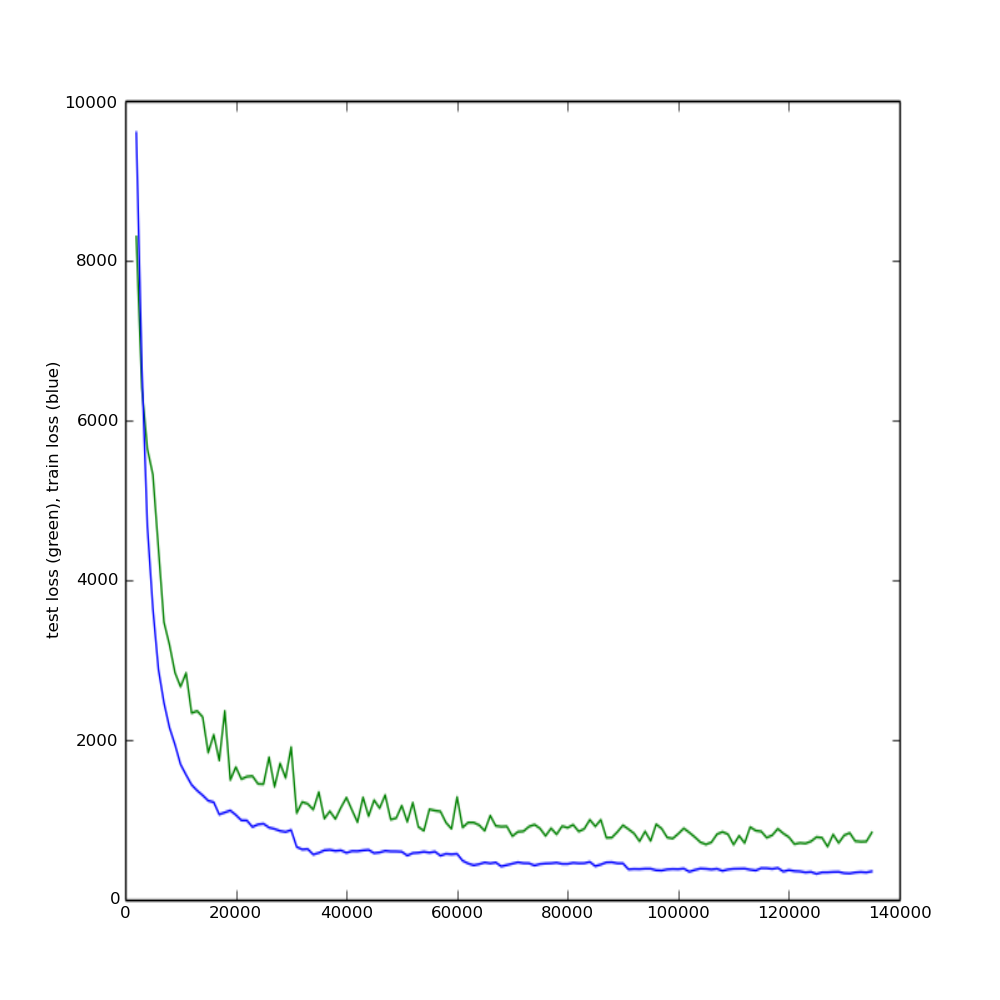
\includegraphics[width=0.3\textwidth]{images/regression/test_loss_26_135000}&
    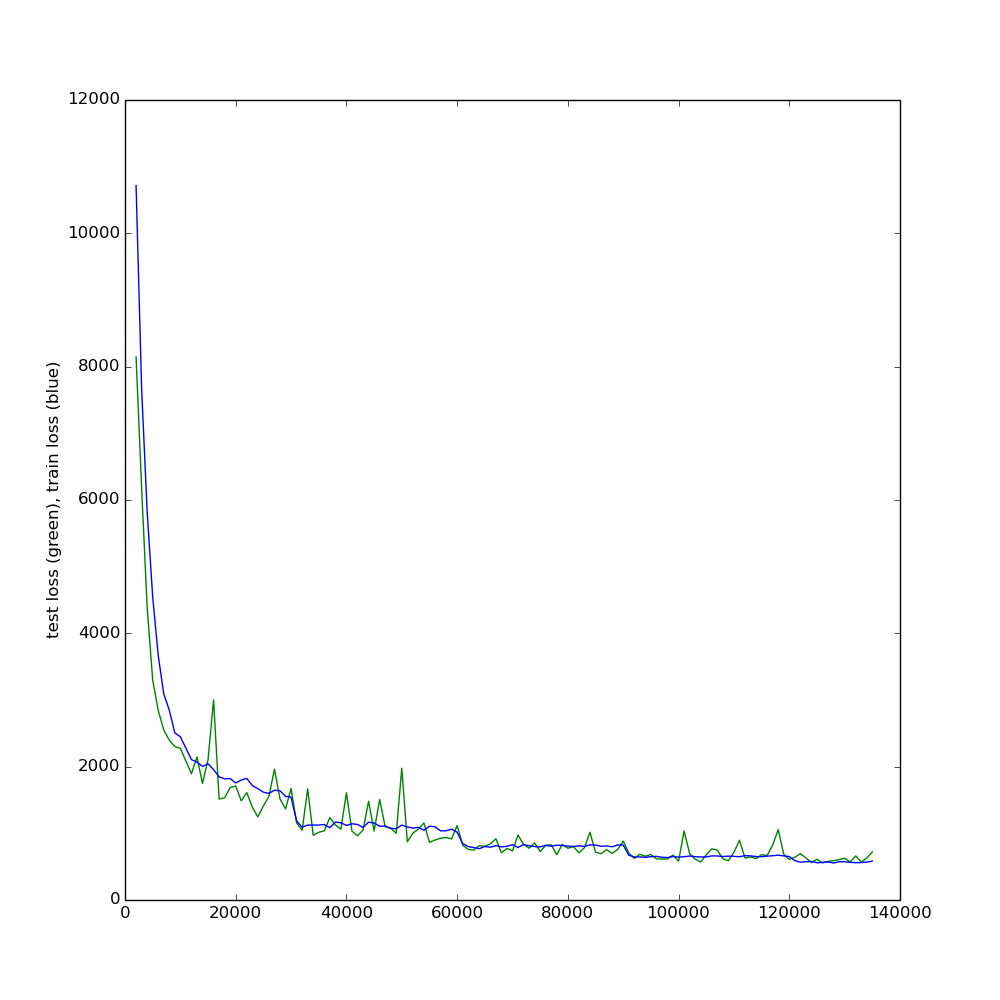
\includegraphics[width=0.3\textwidth]{images/regression/test_loss_37_135000}&
    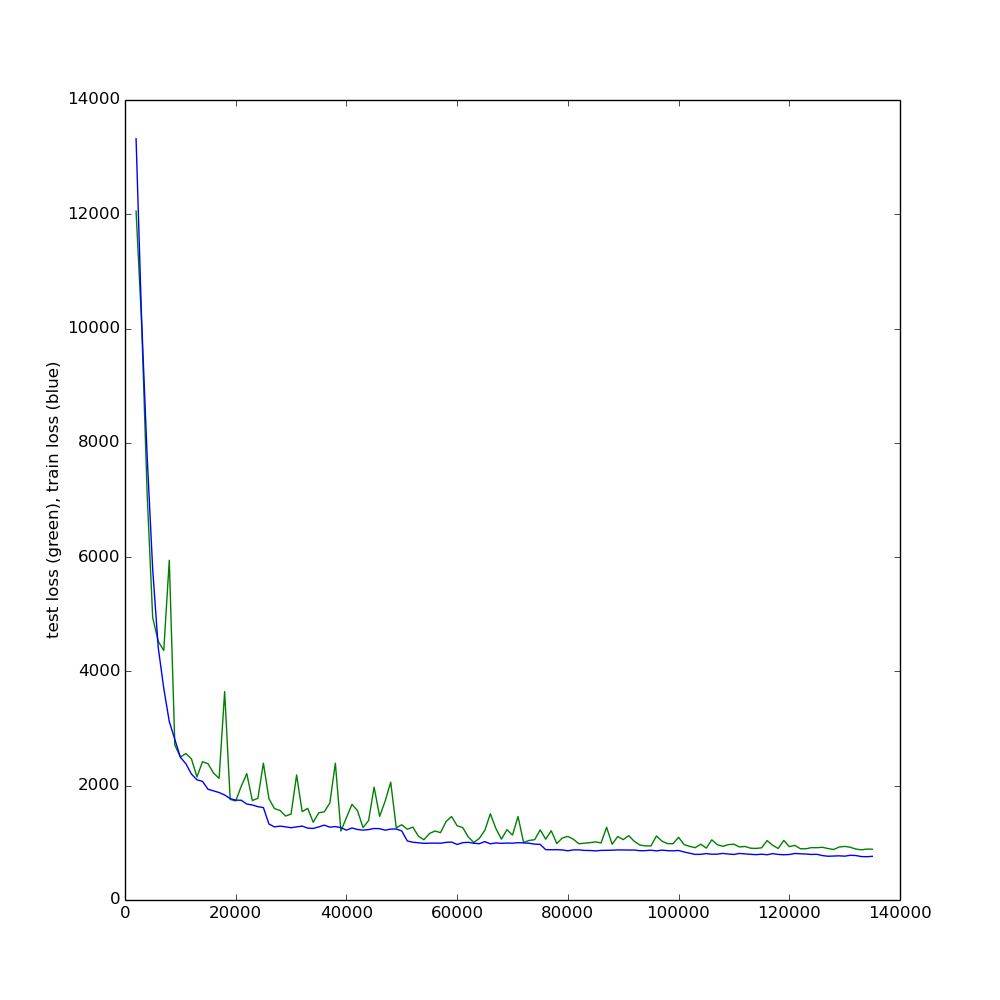
\includegraphics[width=0.3\textwidth]{images/regression/test_loss_30_135000}\\
\end{tabular}
\caption{Loss Function for 135 000 iterations.}
\label{1apploss}
\label{2apploss}
\label{3apploss}
\end{figure}

\begin{figure}[htb]
\centering
\begin{tabular}{ccc}
    a) First approach & b) Second approach & c) Third approach \\
    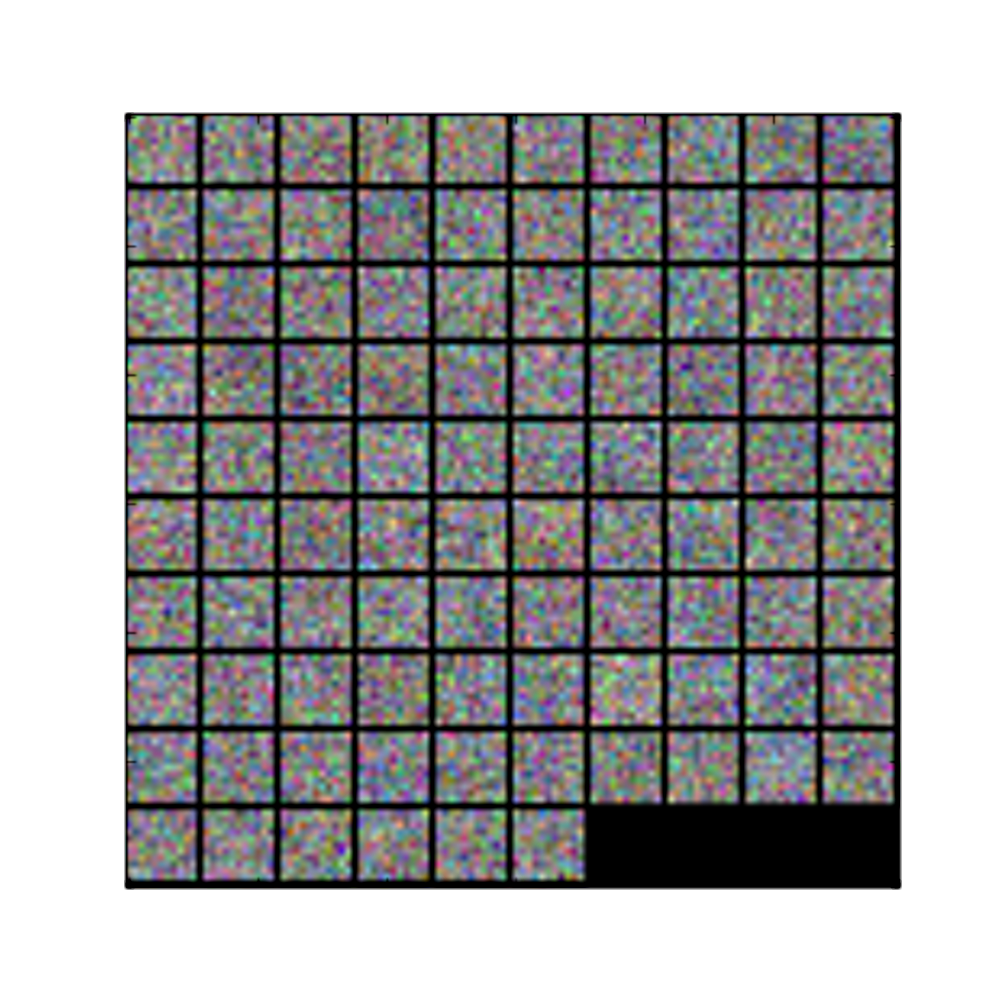
\includegraphics[width=0.3\linewidth]{images/regression/conv1_26_135000}&
    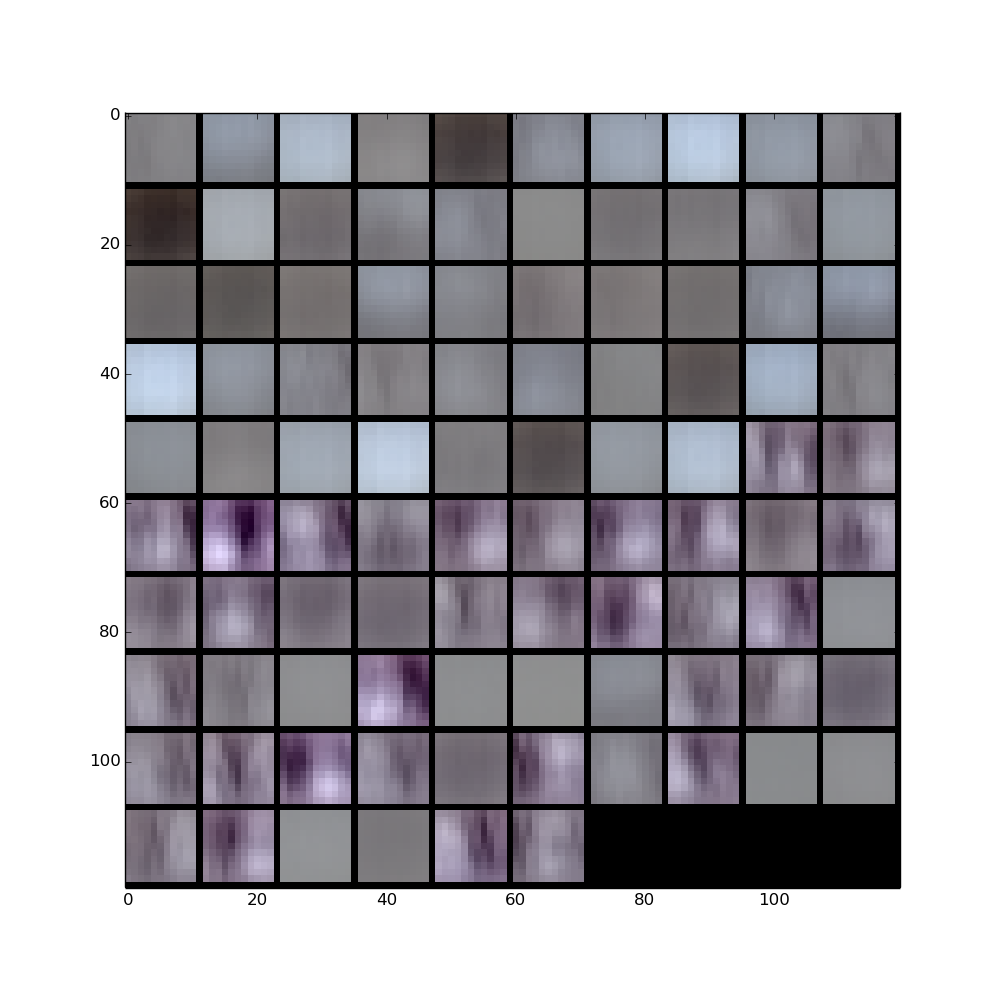
\includegraphics[width=0.3\linewidth]{images/regression/conv1_37_135000}&
    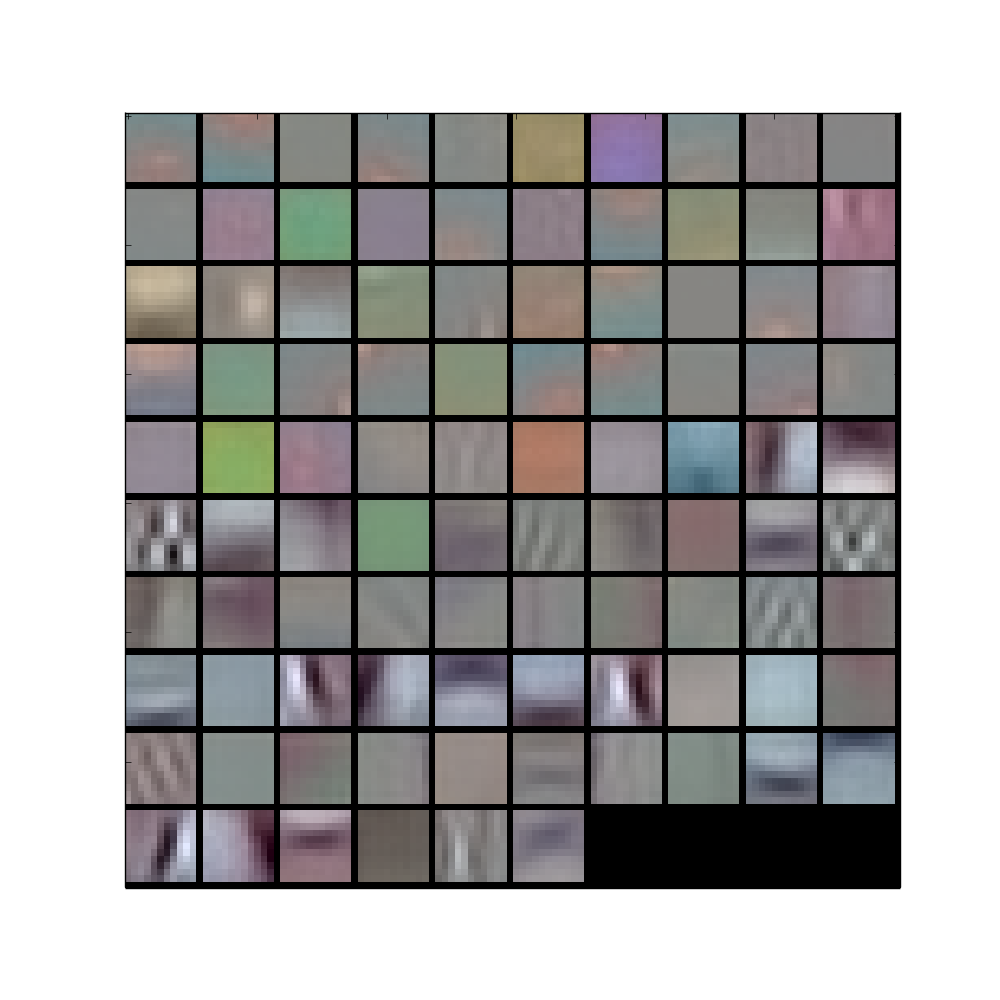
\includegraphics[width=0.3\linewidth]{images/regression/conv1_30_135000}\\
\end{tabular}
\caption{Conv1 filters after 135 000 iterations.}
\label{1appfilter}
\label{2appfilter}
\label{3appfilter}
\end{figure}

The best results regarding the loss values on the train and test datasets were achieved with the second approach. After 148000 iterations, the prediction errors are centered Gaussian-like distributions with a standard deviation of 12.4 meters on X and 20.6 meters on Y. Considering that performing this operation with the human brain is found to be challenging for images from a natural environment, the resulting precision is very acceptable. The labels were displayed to be compared to the predicted positions (fig.~\ref{map}.a and b). The red and green dots represent the original labels and the blue and purple dots represent the predicted labels. The error between X and Y coordinates of the predicted and original labels was also plotted on fig.~\ref{map}.c and was found to be centered on the origin without significant bias.

\begin{figure}[htb]
\centering
\begin{tabular}{p{0.3\textwidth}p{0.3\textwidth}p{0.3\textwidth}}
    %a) Overhead map image with a sample boat path & 
    a) Map of original labels & 
    b) Map of predicted labels&
    c) 2D error of the predicted label position
    \\
    %\bmvaHangBox{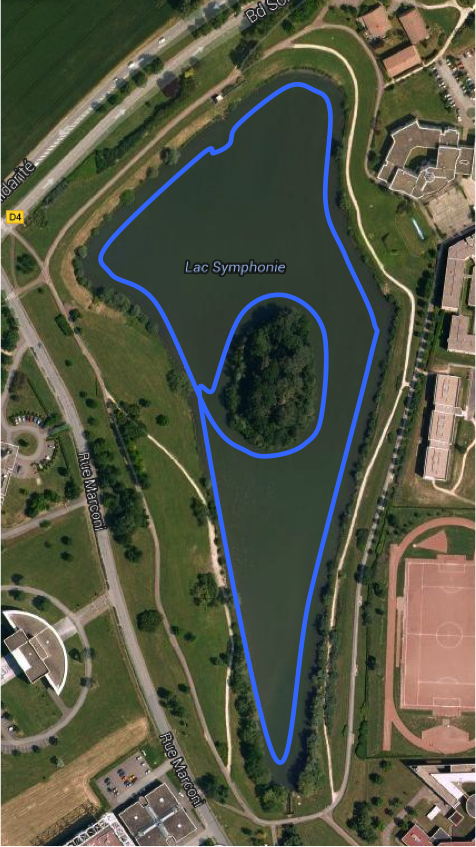
\includegraphics[height=0.4\textwidth]{images/lac}}& 
    \bmvaHangBox{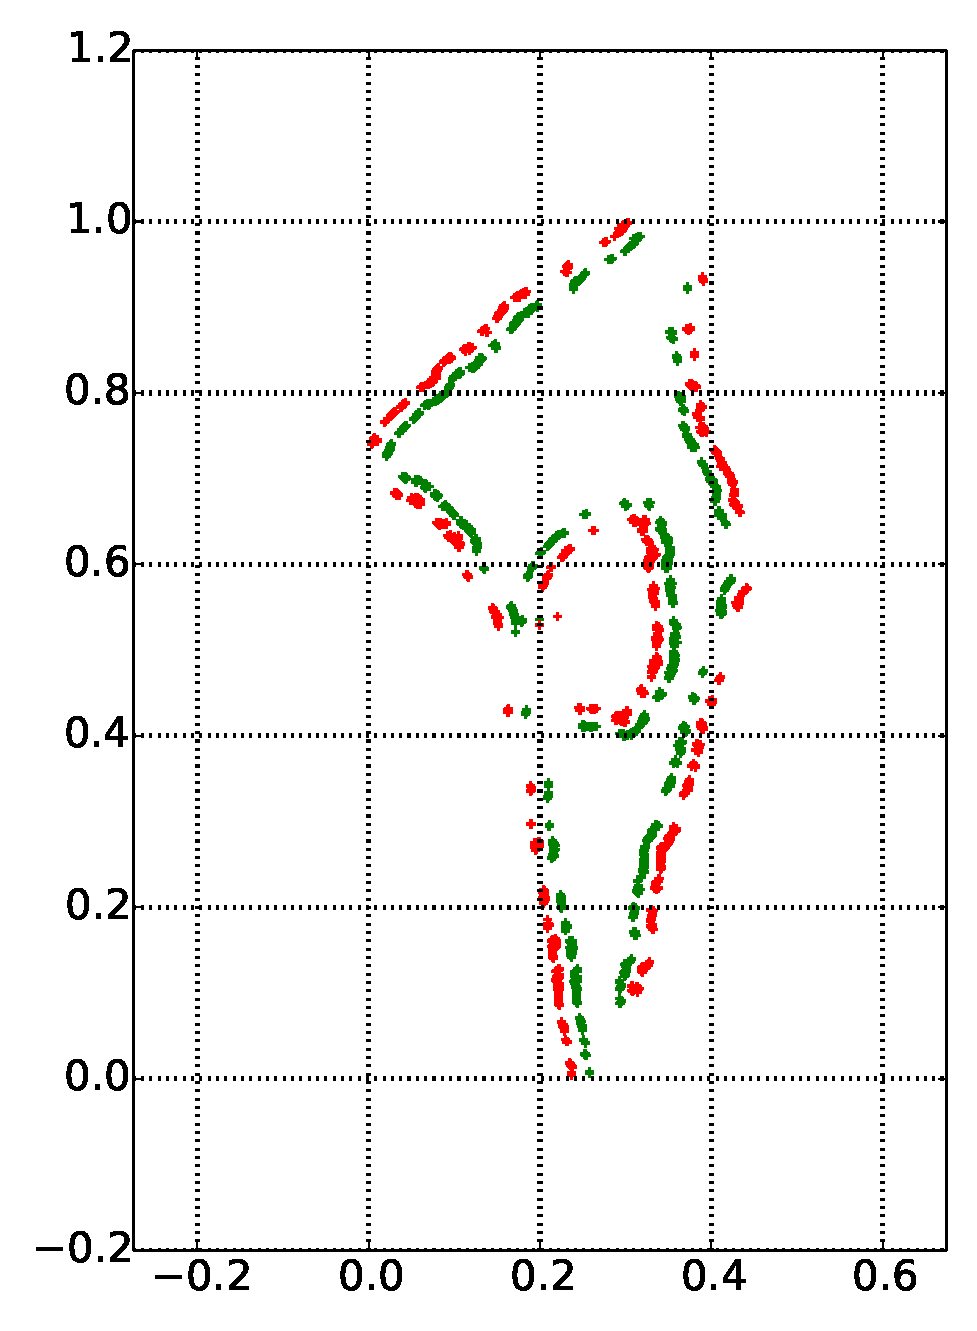
\includegraphics[height=0.4\textwidth]{images/regression/lake_labels_twopoints}} & 
    \bmvaHangBox{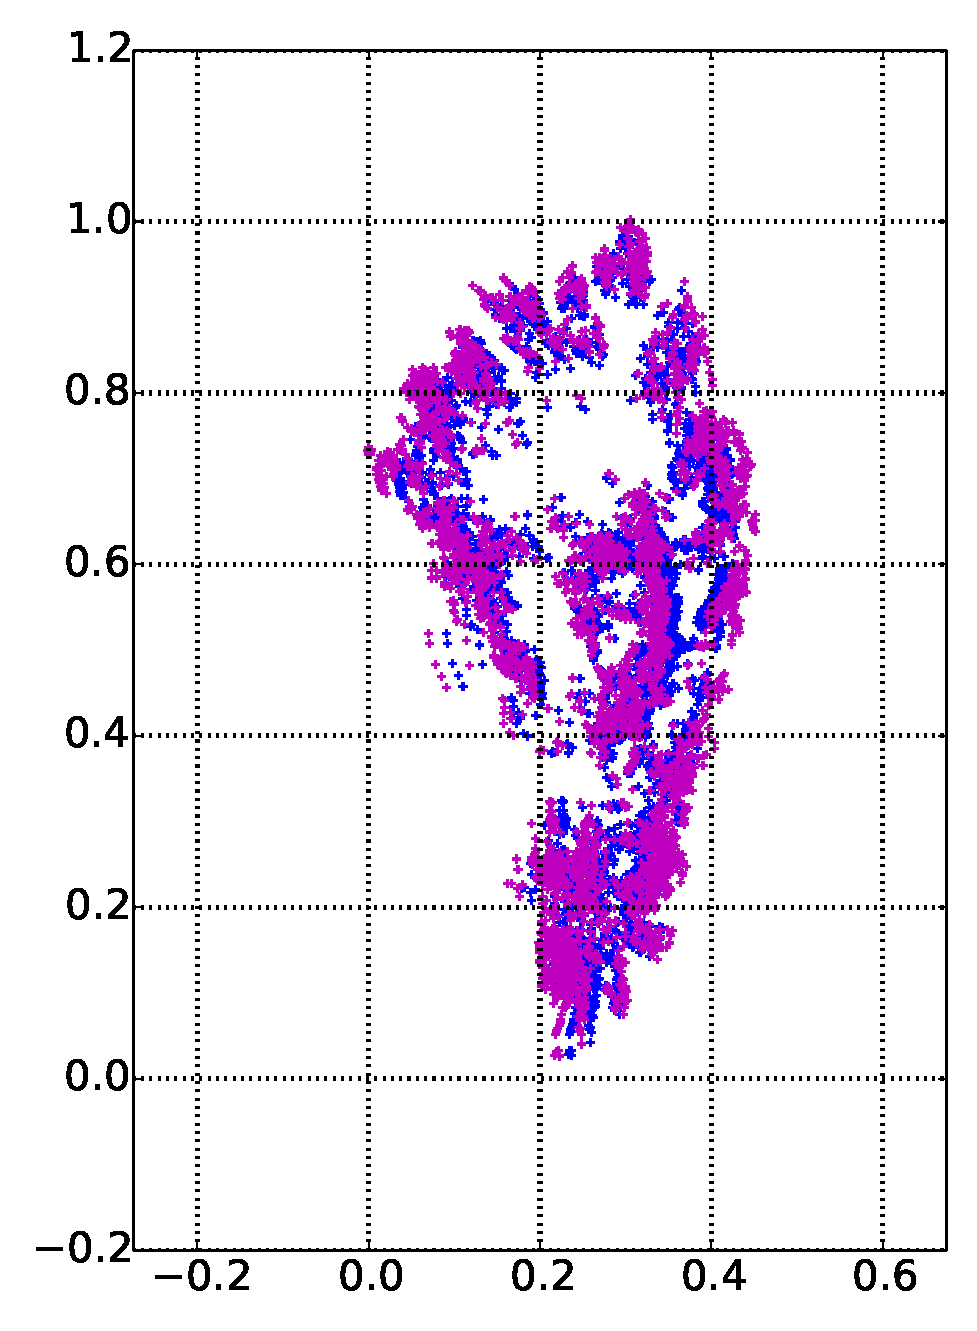
\includegraphics[height=0.4\textwidth]{images/regression/lake_prediction_twopoints}}&
    \bmvaHangBox{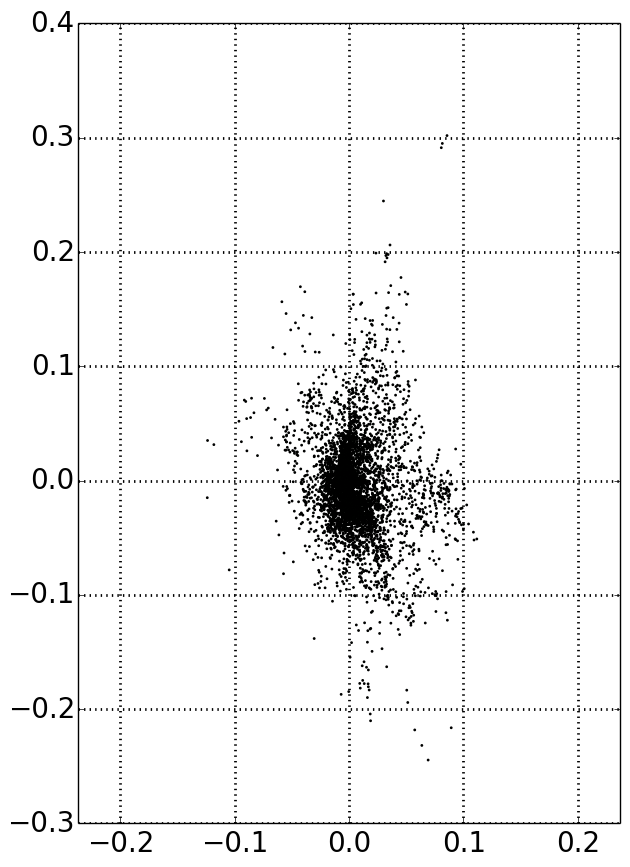
\includegraphics[height=0.4\textwidth]{images/regression/error}}\\
    \\
\end{tabular}
\caption{Map of predicted positions and original labels.}
\label{map}
\label{lake}
\end{figure}

% \begin{figure}[htb]
% \centering
% \begin{tabular}{p{0.3\textwidth}cp{0.3\textwidth}}
%     \bmvaHangBox{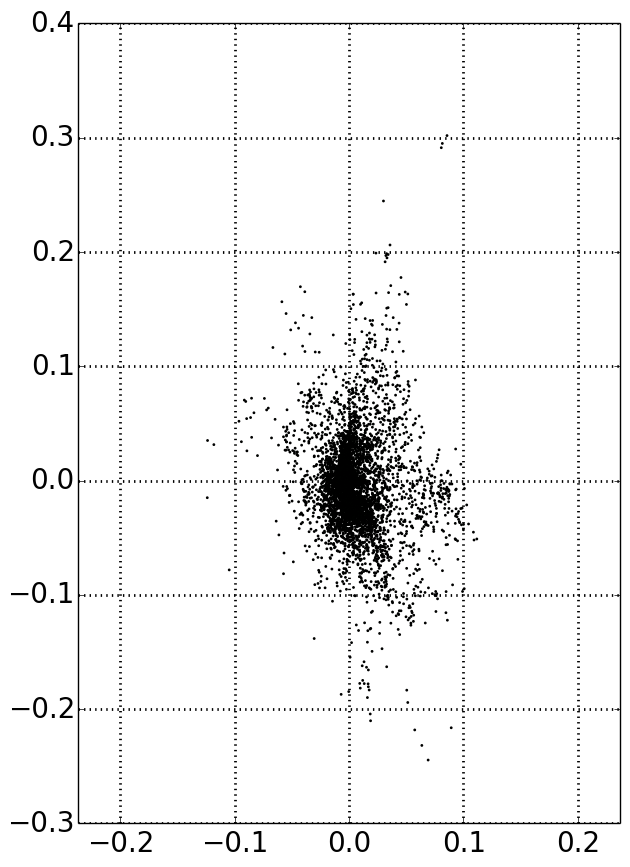
\includegraphics[height=0.3\textwidth]{images/regression/error}}\\
% \end{tabular}
% \caption{Error between X and Y coordinates of predicted and original labels.}
% \label{errormap}
% \end{figure}
